\documentclass[12pt,a4paper,oneside]{report}
\usepackage{indentfirst}
\usepackage{times}
\usepackage[ddmmyyyy,hhmmss]{datetime}
\setlength\parindent{1cm}
\renewcommand{\baselinestretch}{1.50}\normalsize
\usepackage{anysize}
\marginsize{1.25in}{.75in}{1in}{1in}
\usepackage{graphics}
\usepackage[toc,page]{appendix}
\usepackage{graphicx}
\usepackage{url}
\usepackage{epsfig}
\usepackage[fleqn]{amsmath}
\usepackage{amsfonts}
\usepackage{textcomp}
\usepackage{graphicx}
\usepackage{setspace}
\usepackage{fancyhdr}
\usepackage{truncate}
\usepackage{nomencl} 
\usepackage{acronym}
\usepackage{array}
\usepackage{caption}\usepackage{subcaption}
\usepackage{subfig}
\usepackage[overload]{textcase}
\usepackage{listings}
\renewcommand{\nomname}{List of Abbreviations}
\usepackage{makeidx}
\makeindex
\makenomenclature
\newcommand{\quotes}[1]{``#1''}
\usepackage{titlesec}
\titleformat{\chapter}[display]
{\normalfont\Large\bfseries\centering}
{\chaptertitlename\ \thechapter}{15pt}{\LARGE}
\titleformat{\section}{\large\bfseries}{\thesection}{1em}{}
\titleformat{\subsection}{\normalsize\bfseries}{\thesubsection}{1em}{}
\renewcommand{\chaptermark}[1]{\markboth{ \emph{#1}}{}}

\printnomenclature[5em]
\pagestyle{fancy}
%\headheight 1pt
	\renewcommand{\footrulewidth}{1.2pt}
\renewcommand{\headrulewidth}{1.2pt}
\rhead{\scriptsize {\leftmark}}

\lhead{\small{College of Engineering, Cherthala \;\;\;\;\;\;\;\;\;\;\;\;\;\;\;\;\;\;}}
\rfoot{\thepage}
\cfoot{\empty}
\lfoot{\small{Department of Computer Science \& Engineering}}
%\renewcommand{\figurename}{Fig.}
\begin{document}
\renewcommand\bibname{References}
\begin{titlepage}
\begin{center}
\Large{\textbf{MAJOR PROJECT REPORT ON}}\\
\vspace{.2 in}
\begin{singlespace}
\LARGE{\textbf{Continuous Integration Pipeline Implementation for Tech11Software }}\\
\end{singlespace}
\vspace{.2 in}
\Large{\textit{Submitted By }}\\
\Large{\textit{\textbf{ASWIN G SUGUNAN }\textbf{(Reg.No . 12143605)}}} \\
\Large{\textit{\textbf{JEFFIN JACOB  }\textbf{(Reg.No . 12143611)}}} \\
\Large{\textit{\textbf{NITIN SURESH }\textbf{(Reg.No . 12143616)}}} \\
\Large{\textit{\textbf{VISHNU BOSE }\textbf{(Reg.No . 12143626)}}} \\
\Large{\textit{\textit{under the guidance of}}}\\
\Large{\textit{\textbf{Mrs. GREESHMA N GOPAL}}}\\
\Large{\textit{(Assistant Professor)}}\\
\Large{\textit{(Computer Science \& Engineering)}}
\vspace{.05in}
\begin{figure}[h]
\begin{center}

\epsfig{width=1 in, file=logo.jpg}
\end{center}
\end{figure}
\begin{singlespace}
\large{\textbf{MARCH 2017}}\\
\vspace{.1in}
\large{\textbf{DEPARTMENT OF COMPUTER SCIENCE AND ENGINEERING\\COLLEGE OF ENGINEERING,CHERTHALA\\ PALLIPPURAM P O, ALAPPUZHA-688541, \\PHONE: 0478 2553416, FAX: 0478 2552714\\http://www.cectl.ac.in}}
\end{singlespace}
\end{center}
\end{titlepage}
\begin{titlepage}
\begin{center}

\large{\textbf{MAJOR PROJECT REPORT ON}}\\
\Large{\textbf{Continuous Integration Pipeline Implementation for Tech11Software}}\\

\large{\textit{Submitted By }}\\
\begin{singlespace}
%\begin{singlespace}
\Large{\textit{\textbf{ASWIN G SUGUNAN }\textbf{(Reg.No . 12143605)}}} \\
\Large{\textit{\textbf{JEFFIN JACOB  }\textbf{(Reg.No . 12143611)}}} \\
\Large{\textit{\textbf{NITIN SURESH }\textbf{(Reg.No . 12143616)}}} \\
\Large{\textit{\textbf{VISHNU BOSE }\textbf{(Reg.No . 12143626)}}} \\

\end{singlespace}
\large{\textit{\textit{under the guidance of}}}\\
\Large{\textit{\textbf{Mrs. GREESHMA N GOPAL}}}\\
\begin{singlespace}
\large{\textit{In partial fulfilment of the requirements for the award of the degree}\\
\large{ \textit{of}}\\
\large{\textit{Bachelor of Technology} }\\
\large{\textit{in}}\\
\large{\textit{Computer Science and Engineering}}\\
\large{\textit{of}}\\
\large{\textit{Cochin University Of Science And Technology}}}\\
\end{singlespace}
\begin{singlespace}
\begin{figure}[h]
\begin{center}

\epsfig{width=1 in, file=logo.jpg}
\end{center}
\end{figure}
\end{singlespace}
\begin{singlespace}
\large{{\textbf{MARCH 2017\\Department of Computer Science and Engineering\\College of Engineering, Cherthala}\\
Pallippuram P O, Alappuzha-688541 \\Phone: 0478 2553416, Fax: 0478 2552714\\http://www.cectl.ac.in}}
\end{singlespace}
\end{center}
\end{titlepage}
\begin{titlepage}
\begin{center}

\large{\textbf{DEPARTMENT OF COMPUTER SCIENCE \& ENGINEERING}}\\
\large{\textbf{COLLEGE OF ENGINEERING CHERTHALA\\ALAPPUZHA-688541}}\\
\end{center}
\begin{figure}[h]
\begin{center}

\epsfig{width=1.5in, file=logo.jpg}
\end{center}
\end{figure}
\begin{center}
\large{\textbf{C E R T I F I C A T E}}\\
\end{center}
\begin{spacing}{1.5}
This is to certify that, the major project report submitted by \newline Name: \hspace{300pt} Date:\today\newline Reg.No:\newline
On \textbf{\textit{Continuous Integration Pipeline Implementation for Tech11Software}}
 in partial fulfillment of the requirements for the award of the degree, \textbf{B. Tech. Computer Science  \& Engineering } of \textbf{Cochin University of Science \& Technology}.
\end{spacing}
\begin{tabbing}
xxxxxxxxxxxxxxxxxxxxxxxxxxxxxxxxxxxxxx\= xxxxxxxxxxxxxxxxxxxx\= \kill
\hspace{.15in}{\bf Guide} \>\hspace{-.7in}{\bf Co-ordinator}\hspace{1.45in}{\bf  HoD  } \\
\end{tabbing}
\begin{tabbing}
xxxxxxxxxxxxxxxxxxxxxxxxxxxxxxxxxxxxxx\= xxxxxxxxxxxxxxxxxx\= \kill
%\vspace{0.3in}\\
\hspace{.15in}{\bf{Mrs. Greeshma N Gopal}}   \>\hspace{-.7in}{\bf Mr. Muhammed Ilyas H} \hspace{.55 in}{\bf Dr. Preetha Theresa Joy}\\
\hspace{.15in}Assistant Professor    \>\hspace{-.7in}Assistant Professor\>\hspace{.20in}Professor\\
\hspace{.1in} Computer Science\&Engg    \>\hspace{-.75in}    Computer Science\&Engg \>\hspace{.15in}    Computer Science\&Engg\\

\end{tabbing}
\end{titlepage}


\renewcommand*\thesection{\thechapter.\arabic{section}}
%\pagenumbering{arabic}
%\addtocounter{page}{4}


\begin{titlepage}
\pagenumbering{arabic}
%\addtocounter{page}{4}
\setcounter{page}{4}
\section*{\begin{center} \Large{ACKNOWLEDGEMENT }\end{center}}

\thispagestyle{plain}


%{$\;\;\;\:$}
\par
We take this opportunity to express our sincere gratitude to the people who have been
instrumental in the successful completion of our major project.
For every endeavour in our life, the help of the Lord has always followed. We have yet
again experienced his loving kindness while preparing for this project.
We would like to express our sincere thanks to the Principal, \textbf{Dr. Mini M. G}, for her
valuable support and advice. We would also like to thank our Head Of Computer Science
Department, \textbf{Dr. Preetha Teresa Joy} (Professor, Computer Science and Engineering Department) for her support. We express our heartfelt gratitude to
our project coordinator, \textbf{Mr. Muhammed Ilyas H} (Assistant Professor, Computer Science and Engineering Department) for his valuable help and support. We would also like to thank our project Guide,
\textbf{Mrs. Greeshma N Gopal} (Assistant Professor, Department of Computer Science) for her support and
guidance. Special thanks to \textbf{Mr. Gireesh N Gopal} (Technical Advisor at Tech11 Software) for introducing us to Continuous Integration and his guidance.
We are indebted to all teaching and non-teaching staff of the Department of Computer
Science and Engineering, friends and family for their co-operation and support, with out which
we could never have completed the project this well. \\
\end{titlepage}
\newpage

\section*{\begin{center}\Large ABSTRACT\end{center}}
\thispagestyle{empty}
\par
\hspace{0.1in}
{
Software development, as we know it today, is a demanding area of business with it's fast-changing customer requirements, pressures of an ever shorter time to-market, and unpredictability of market. With the shift towards modern continuous deployment pipelines, releasing new software versions early and often has become a concrete option also for an ever growing number of practitioners. \par Continuous delivery is a software development practice where new features are made available to end users as soon as they have been implemented and tested. In such a setting, a key technical piece of infrastructure is the development pipeline that consists of various tools and databases, where features are made available from development to deployment and then further to use.
\tableofcontents
\pagenumbering{roman}
\listoffigures


\def\addsymbol #1: #2#3{\;\;\;\;\;\;\;\;\;\;\;\;\;\;\;\;\;\;\;\;\;\;\;$#1$ \> \;\;\;\;\;\;\;\;\;\;\;\;\;\;\;\;\;\;\;\;\;\;\;\;\;\; \parbox{5in}{#2}\\}


\renewcommand*\thesection{\thechapter.\arabic{section}}
\newpage
\pagestyle{fancy}
\headheight 26pt
\renewcommand{\footrulewidth}{1.2pt}
\renewcommand{\headrulewidth}{1.2pt}
\rhead{\scriptsize {\leftmark}}
%\chead{Middle top}
\lhead{\small{College of Engineering, Cherthala \;\;\;\;\;\;\;\;\;\;\;\;\;\;\;\;\;\;}}
\rfoot{\thepage}
\cfoot{\empty}
\lfoot{\small{Department of Computer Science \& Engineering}}


\chapter{INTRODUCTION}
\label{intro}
\pagenumbering{arabic}
\setcounter{page}{1}
%\hspace{0.1in}
Continuous integration is the practice where members of a development team integrate their work frequently. Usually each of them integrates at least daily, which leads to multiple integrations per day. To detect errors, each integration is verified by an automated build and test. This approach is generally found to lead to a significant reduction of integration problems, which in turn allows teams to develop cohesive software even in a limited time frame.
\section{PURPOSE}
\par The objective of the project is to put in place a Continuous Integration framework for product
development activities of Tech11 Softwares. This would enable the Tech11 team to rapidly bring a
product change or feature to production gaining market advantage.
\par
This activities of this project will involve accessing different CI integration approaches and
solutions available, identify the feasibility of those solution by doing POCs and demos, fine tune the
final solution and set up the CI infrastructures, educate the developers on CI culture.

\section{PRODUCT SCOPE}
\par  The scope of the system is to help software developers to ensure new features are made available as soon as the program has been
implemented and tested. This product also helps in reducing the time needed to develop a software and also acts a guideline for future software developments


\chapter{OVERALL DESCRIPTION}
\section{PRODUCT PERSPECTIVE}
\par
Continuous Integration is based on continuous performance of acts of integration of
source code, testing, building and deployment in response to each change to the source code of
the project submitted by the developer and for the use of tools for support of the development
and testing by compliance with the established procedure automatically. The proposed system
directs the user (developers) for time and cost effective production and solves majority of the
Integration hell problem. \par
Integration Hell refers to the point in production when members on a delivery team integrate
their individual code. In traditional software development environments, this integration
process is rarely smooth and seamless, instead resulting in hours or perhaps days of fixing the
code so that it can finally integrate. Continuous Integration (CI) aims to avoid this completely
by enabling and encouraging team members to integrate frequently (e.g., hourly, or at least
daily).
%\subsection{Current system}
%\par

\subsection{Proposed System}
\par 
The Proposed system is to help software developers to ensure new features are made
available as soon as the program has been implemented and tested. This product also helps in
reducing the time needed to develop a software and also acts a guideline for future software
developments.
\section{SOLUTION FUNCTION}

\par Continuous integration – the practice of frequently integrating one's new or changed code with the existing code repository. Integration should occur frequently enough that no intervening window remains between commit and build, and such that no errors can arise without developers noticing them and correcting them immediately. Normal practice is to trigger these builds by every commit to a repository, rather than a periodically scheduled build. The practicalities of doing this in a multi-developer environment of rapid commits are such that it is usual to trigger a short time after each commit, then to start a build when either this timer expires, or after a rather longer interval since the last build. Many automated tools offer this scheduling automatically.

\begin{itemize}
\item \textbf{Version Control}

\par This practice advocates the use of a revision control system for the project's source code. All artifacts required to build the project should be placed in the repository. In this practice and in the revision control community, the convention is that the system should be buildable from a fresh checkout and not require additional dependencies.  Extreme Programming  mentions that where branching is supported by tools, its use should be minimised. Instead, it is preferred for changes to be integrated rather than for multiple versions of the software to be maintained simultaneously. 
\item \textbf{Artifact Manager}
\par 
While many developers have adopted Maven as a build tool, most have yet to understand the importance of maintaining a repository manager both to proxy remote repositories and to manage and distribute software artifacts. A repository stores two types of artifacts: releases and snapshots. Release repositories are for stable, static release artifacts and snapshot repositories are frequently updated repositories that store binary software artifacts from projects under constant development. While it is possible to create a repository which serves both release and snapshot artifacts, repositories are usually segmented into release or snapshot repositories serving different consumers and maintaining different standards and procedures for deploying artifacts. Much like the difference between a production network and a staging network, a release repository is considered a production network and a snapshot repository is more like a development or a testing network. While there is a higher level of procedure and ceremony associated with deploying to a release repository. Snapshot artifacts can be deployed and changed frequently without regard for stability and repeatability concerns.
\item \textbf{Continuous Integration Handler}
\par While there are many tools, we focus on one of the most popular, Jenkins CI. This is one of the more popular (open source) tools available. Jenkins CI (the continuation of a product formerly called Hudson) allows continuous integration builds in the following ways:
\begin{itemize}
\item It integrates with popular build tools (ant, maven, make) so that it can run the appropriate build scripts to compile, test and package within an environment that closely matches what will be the production environment
\item It integrates with version control tools, including Subversion, so that different projects can be set up depending on projection location within the trunk.
\item It can be configured to trigger builds automatically by time and/or changeset. (i.e., if a new changeset is detected in the Subversion repository for the project, a new build is triggered.)
\item It reports on build status. If the build is broken, it can be configured to alert individuals by email.
\end{itemize}


 \item  \textbf{Test Automator}
\par In software testing, test automation is the use of special software (separate from the software being tested) to control the execution of tests and the comparison of actual outcomes with predicted outcomes. Test automation can automate some repetitive but necessary tasks in a formalized testing process already in place, or perform additional testing that would be difficult to do manually. Test automation is critical for continuous delivery and continuous testing. There are many approaches to test automation, however below are the general approaches used widely:

\begin{itemize}
\item Graphical user interface testing. A testing framework that generates user interface events such as keystrokes and mouse clicks, and observes the changes that result in the user interface, to validate that the observable behavior of the program is correct.
\item API driven testing. A testing framework that uses a programming interface to the application to validate the behaviour under test. Typically API driven testing bypasses application user interface altogether. It can also be testing public (usually) interfaces to classes, modules or libraries are tested with a variety of input arguments to validate that the results that are returned are correct.
\end{itemize}


\item \textbf{Continuous Deployment}
\par Continuous deployment is the next step of continuous delivery: Every change that passes the automated tests is deployed to production automatically. Continuous deployment should be the goal of most companies that are not constrained by regulatory or other requirements.

\end{itemize}

 
\section{OPERATING ENVIRONMENT}
The system is expected to be operated in Linux as well as in windows with the support of
respective JRE (Java Runtime Environment). This system based project is completely platform
independent. The most important requirement is the Internet connection. This tool is coded
using JDK 1.6.
\section{GANTT CHART} 
\par Gantt chart is a graphical representation of allocation of resources to the activities. Here
our resource is time. A Gantt chart is a type of bar chart that illustrates a project schedule.
Gantt charts illustrate the start and finish dates of the terminal elements and summary elements
of a project. Terminal elements and summary elements comprise the work breakdown structure
of the project. Some Gantt charts also show the dependency (i.e., precedence network)
relationships between activities.
\par Gantt charts have become a common technique for representing the phases and activities
of a project work breakdown structure (WBS), so they can be understood by a wide audience.
Although a Gantt chart is useful and valuable for small projects that fit on a single sheet or
screen, they can become quite unwieldy for projects with more than about 30 activities. Larger
Gantt charts may not be suitable for most computer displays. A related criticism is that Gantt
charts communicate relatively little information per unit area of display. That is, projects are
often considerably more complex than can be communicated effectively with a Gantt chart.
Although project management software can show schedule dependencies as lines between activities,
displaying a large number of dependencies may result in a cluttered or unreadable
chart.
\par Because the horizontal bars of a Gantt chart have a fixed height, they can misrepresent
the time-phased workload (resource requirements) of a project, which may cause confusion especially
in large projects. A related criticism is that all activities of a Gantt chart show planned
workload as constant. In practice, many activities (especially summary elements) have front loaded
or back-loaded work plans, so a Gantt chart with percent-complete shading actually may
lead to mis-communications on the true schedule performance status.
\newpage
\begin{figure}[h]
\begin{center}
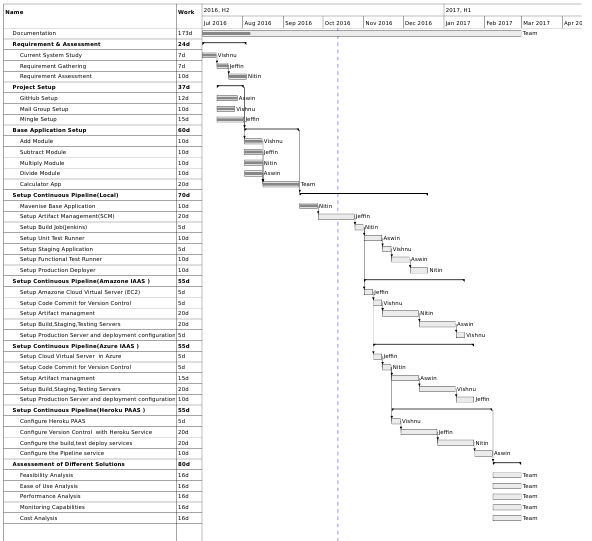
\includegraphics[scale=1.1]{gnt.png}
\caption{Gantt chart}
\label{Gantt chart}
\end{center}
\end{figure}
\newpage


\par
\section{EXTERNAL INTERFACE REQUIREMENTS}
This system based software can be used in any operating system such as Microsoft Windows, Linux or any kind of user application interface, since it is platform independent.

\subsection{User Interface}
Interface hardware shall be encapsulated in a set of classes that isolate hardware specifications from the rest of the software. In particular, interfaces for specific hardware boards shall be implemented as derived classes of an abstract class.
\\

\subsection{Network Requirements}  
\begin{itemize}
\item Systems need minimum speed internet connection.
\end{itemize}
\subsection{Software Requirements}
\begin{itemize}
\item Git
\item Jenkins
\item Checkstyle
\item Findbugs
\item Heroku
\end{itemize}
\chapter{SYSTEM DESIGN}
\section{MODULES}
\subsection{Version Control}

\par This practice advocates the use of a revision control system for the project's source code. All artefacts required to build the project should be placed in the repository. In this practice and in the revision control community, the convention is that the system should be buildable from a fresh checkout and not require additional dependencies.  Extreme Programming  mentions that where branching is supported by tools, its use should be minimised. Instead, it is preferred for changes to be integrated rather than for multiple versions of the software to be maintained simultaneously. 
\subsection{Artifact Manager}
\par 
While many developers have adopted Maven as a build tool, most have yet to understand the importance of maintaining a repository manager both to proxy remote repositories and to manage and distribute software artifacts. A repository stores two types of artifacts: releases and snapshots. Release repositories are for stable, static release artifacts and snapshot repositories are frequently updated repositories that store binary software artifacts from projects under constant development. While it is possible to create a repository which serves both release and snapshot artifacts, repositories are usually segmented into release or snapshot repositories serving different consumers and maintaining different standards and procedures for deploying artifacts. Much like the difference between a production network and a staging network, a release repository is considered a production network and a snapshot repository is more like a development or a testing network. While there is a higher level of procedure and ceremony associated with deploying to a release repository, snapshot artifacts can be deployed and changed frequently without regard for stability and repeatability concerns.\subsection{Continuous Integration Handler}
\par While there are many tools, I will focus on one of the most popular, Jenkins CI. This is one of the more popular (open source) tools available. Jenkins CI (the continuation of a product formerly called Hudson) allows continuous integration builds in the following ways:
\begin{itemize}
\item It integrates with popular build tools (ant, maven, make) so that it can run the appropriate build scripts to compile, test and package within an environment that closely matches what will be the production environment
\item It integrates with version control tools, including Subversion, so that different projects can be set up depending on projection location within the trunk.
\item It can be configured to trigger builds automatically by time and/or changeset. (i.e., if a new changeset is detected in the Subversion repository for the project, a new build is triggered.)
\item It reports on build status. If the build is broken, it can be configured to alert individuals by email.
\end{itemize}

 
\subsection{Test Automator}
\par In software testing, test automation is the use of special software (separate from the software being tested) to control the execution of tests and the comparison of actual outcomes with predicted outcomes. Test automation can automate some repetitive but necessary tasks in a formalized testing process already in place, or perform additional testing that would be difficult to do manually. Test automation is critical for continuous delivery and continuous testing. There are many approaches to test automation, however below are the general approaches used widely:

\begin{itemize}
\item Graphical user interface testing. A testing framework that generates user interface events such as keystrokes and mouse clicks, and observes the changes that result in the user interface, to validate that the observable behavior of the program is correct.
\item API driven testing. A testing framework that uses a programming interface to the application to validate the behaviour under test. Typically API driven testing bypasses application user interface altogether. It can also be testing public (usually) interfaces to classes, modules or libraries are tested with a variety of input arguments to validate that the results that are returned are correct.
\end{itemize}


\subsection{Continuous Deployment}
\par Continuous deployment is the next step of continuous delivery: Every change that passes the automated tests is deployed to production automatically. Continuous deployment should be the goal of most companies that are not constrained by regulatory or other requirements.


\newpage
\section{DATA FLOW DIAGRAMS}
\subsection {Purpose} 
\par The Data Flow Diagram (DFD) is used for classifying system requirements to major transformation that will be come programs in system design. This is starting point of the design phase that functionally decomposes the required specifications down to the lower level of details. It consists of a series of bubbles joint together by lines. Bubbles: Represent the data transformations. Lines: Represent the logic Flow of data. Data can trigger events and can be processed to useful information. Systems analysis recognizes the central goal of data in organizations. This data flow analysis tells a great deal about how organization objectives are accomplished.


\subsection{Description}
\begin{itemize}
\item  Process : Describes how each input data is converted to output data.
\item  Data Store : Describes the repositories of data in a system.
\item   Data Flow : Describes the data flowing between Processes, Data stores, Entities.
\item   Entity : An external entity causing the origin of data.
%\end{itemize}
\begin{figure}[h]
\begin{center}
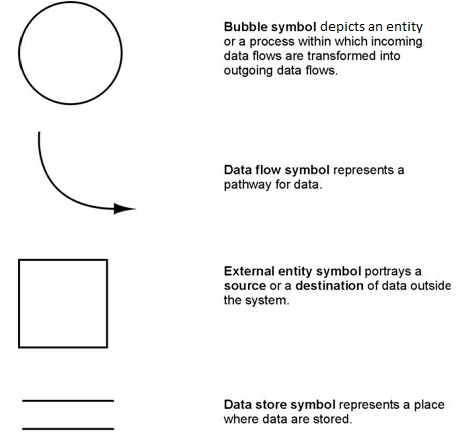
\includegraphics[scale=0.75]{dfd.png}
\caption{Notations used in  DFD}
\label{Notations used in  DFD}
\end{center}
\end{figure}
\end{itemize}
\newpage


\newpage
\subsection{Level 0 DFD}
Level 0 DFD gives a simple information about the overall structure. Here user can commit the changes in the code to the CI server the CI server then feedback the response to the developer
\begin{figure}[h!]
\begin{center}

\hspace{1 in}
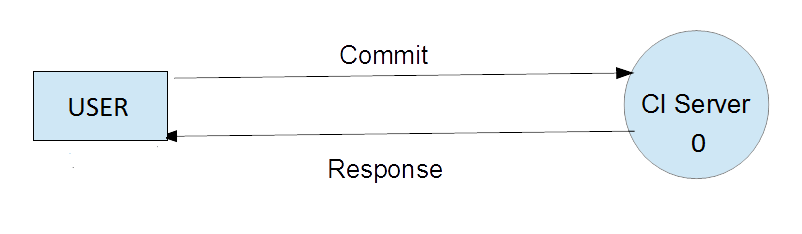
\epsfig{width=4in, file=dfd1.png}
\caption{Level 0 DFD}
\end{center}
\end{figure}
\newpage
\subsection{Level 1 DFD}
The level 1 DFD gives a basic structure of the project indicating the five modules needed to execute the project. The changes of the code is first pushed into the local repository then the changes will be periodically pulled or automatically triggered for each push to the CI server. The response will be feedback to the developer.
\begin{figure}[h]
\begin{center}
\hspace{1 in}
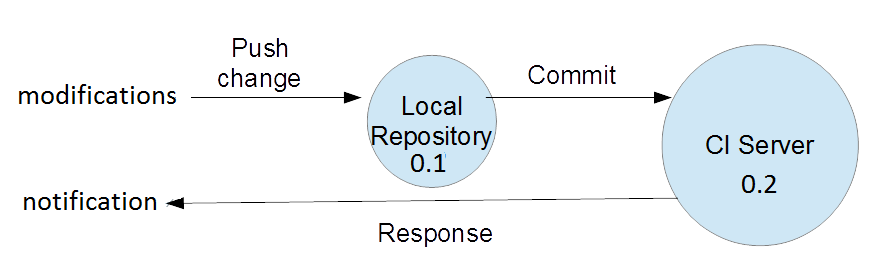
\epsfig{width=4in, file=dfd2.png}
\caption{Level 1.1 DFD}
\end{center}
\vspace{-1.5 in}
\end{figure}

%\begin{figure}[h]
%\begin{center}
%\epsfig{width=5in, file=dfd1_2.jpg}
%\caption{Level 1.1 DFD}
%\end{center}
%\end{figure}
\vspace{100pt}
\subsection{Level 2 DFD}
The level 2 DFD gives a much more advanced idea about the execution. Each of these sections perform unique functions and these are combined together to yield the final product. Developer pushes to a local version control system. then the build request will be sen to the CI handler. the CI handler uses the artifact manager to manage all dependencies and uses a staging server for the deployment.the staging server can use the test runners for testing and production box for product release.
\newpage
\begin{figure}[h]
\begin{center}
\vspace{0.5 in}
\hspace{.0 in}
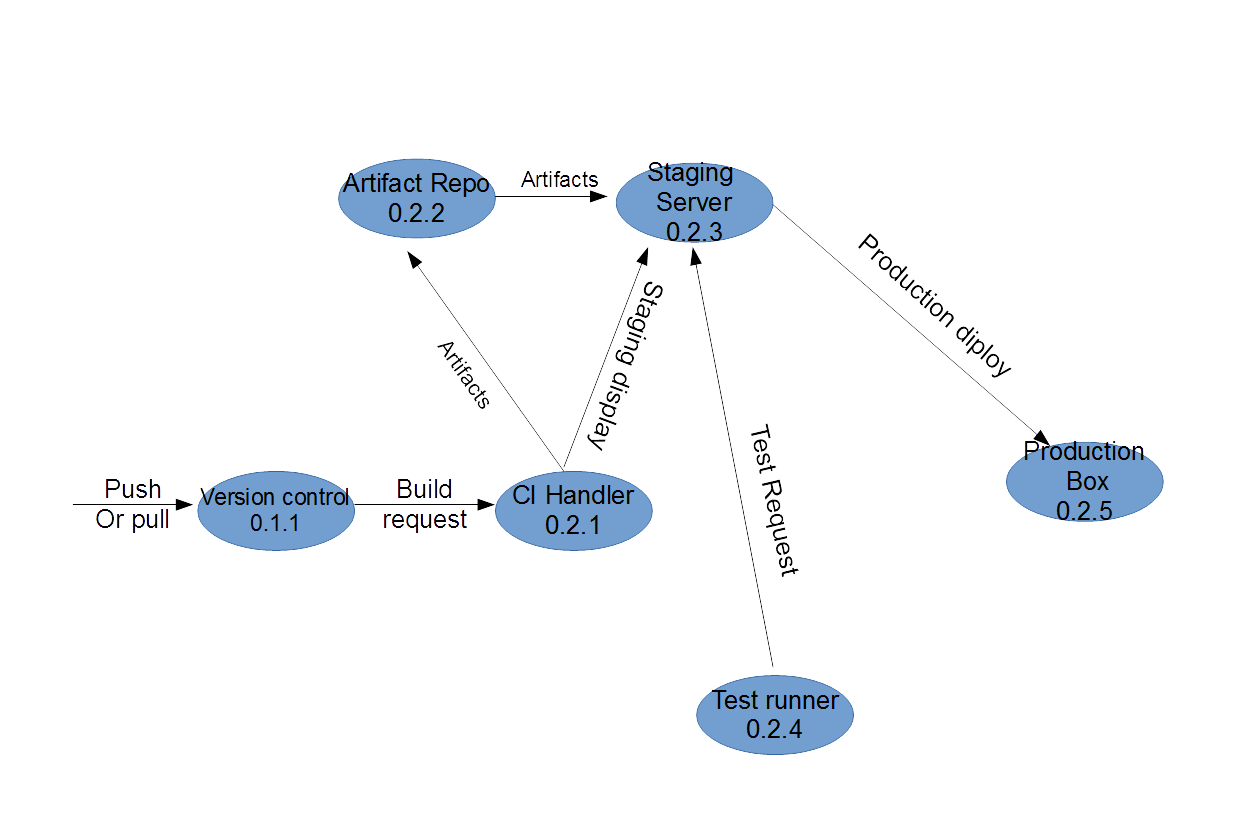
\epsfig{width=6in, file=dfd3.png}
\caption{Level 2.1.1 DFD}
\end{center}

\end{figure}
\newpage
\section{FLOW DIAGRAM}
Flow diagram is a collective term for a diagram representing a flow or set of dynamic relationships in a system. The term flow diagram is also used as a synonym for flowchart, and sometimes as a counterpart of the flowchart.

Flow diagrams are used to structure and order a complex system, or to reveal the underlying structure of the elements and their interaction.
\begin{figure}[h]
\begin{center}

\hspace{.0 in}
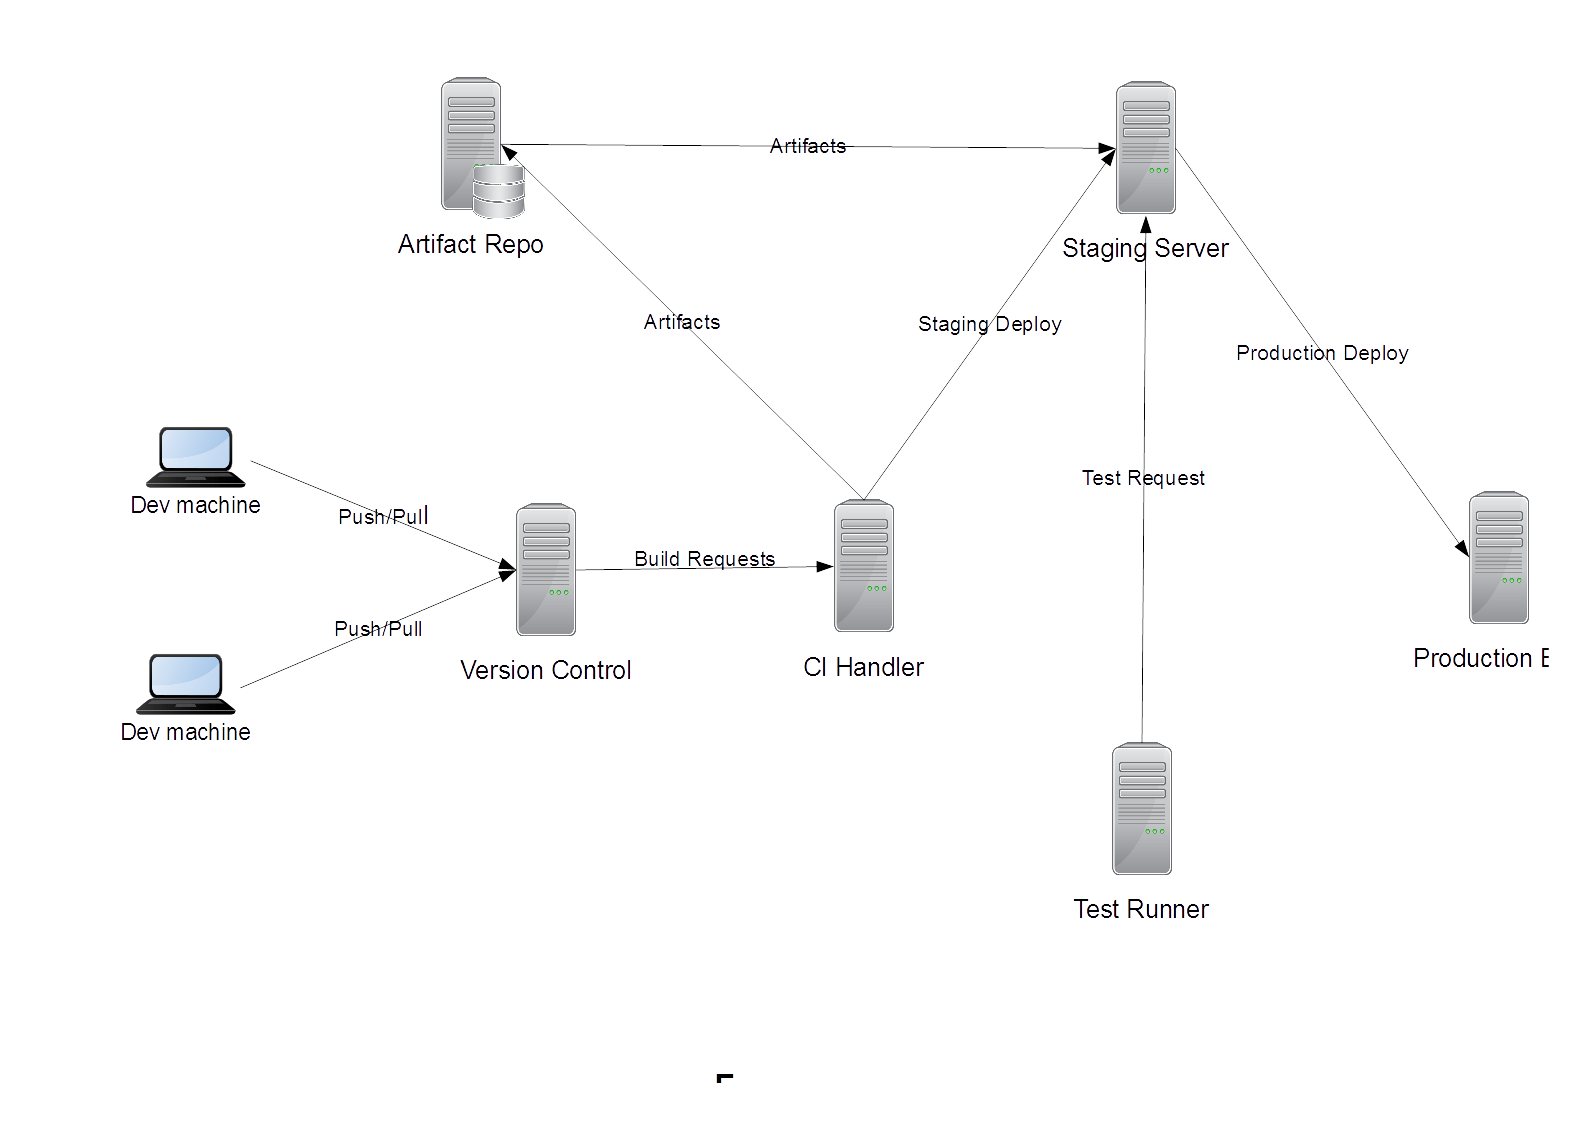
\epsfig{width=6in, file=flow1.png}
\caption{Flow diagram}
\end{center}

\end{figure}
\pagebreak
\section{C.I PIPELINE DIAGRAM}
A Pipeline diagram shows the series of instruction that take place during the execution of the system. The developer push to the git then a build request will be send to the jenkins, it uses nexus SCM for managing the jars also uses the tomcat for staging deploy. tomcat uses selenium test runner.
\begin{figure}[h]
\begin{center}

\hspace{.0 in}
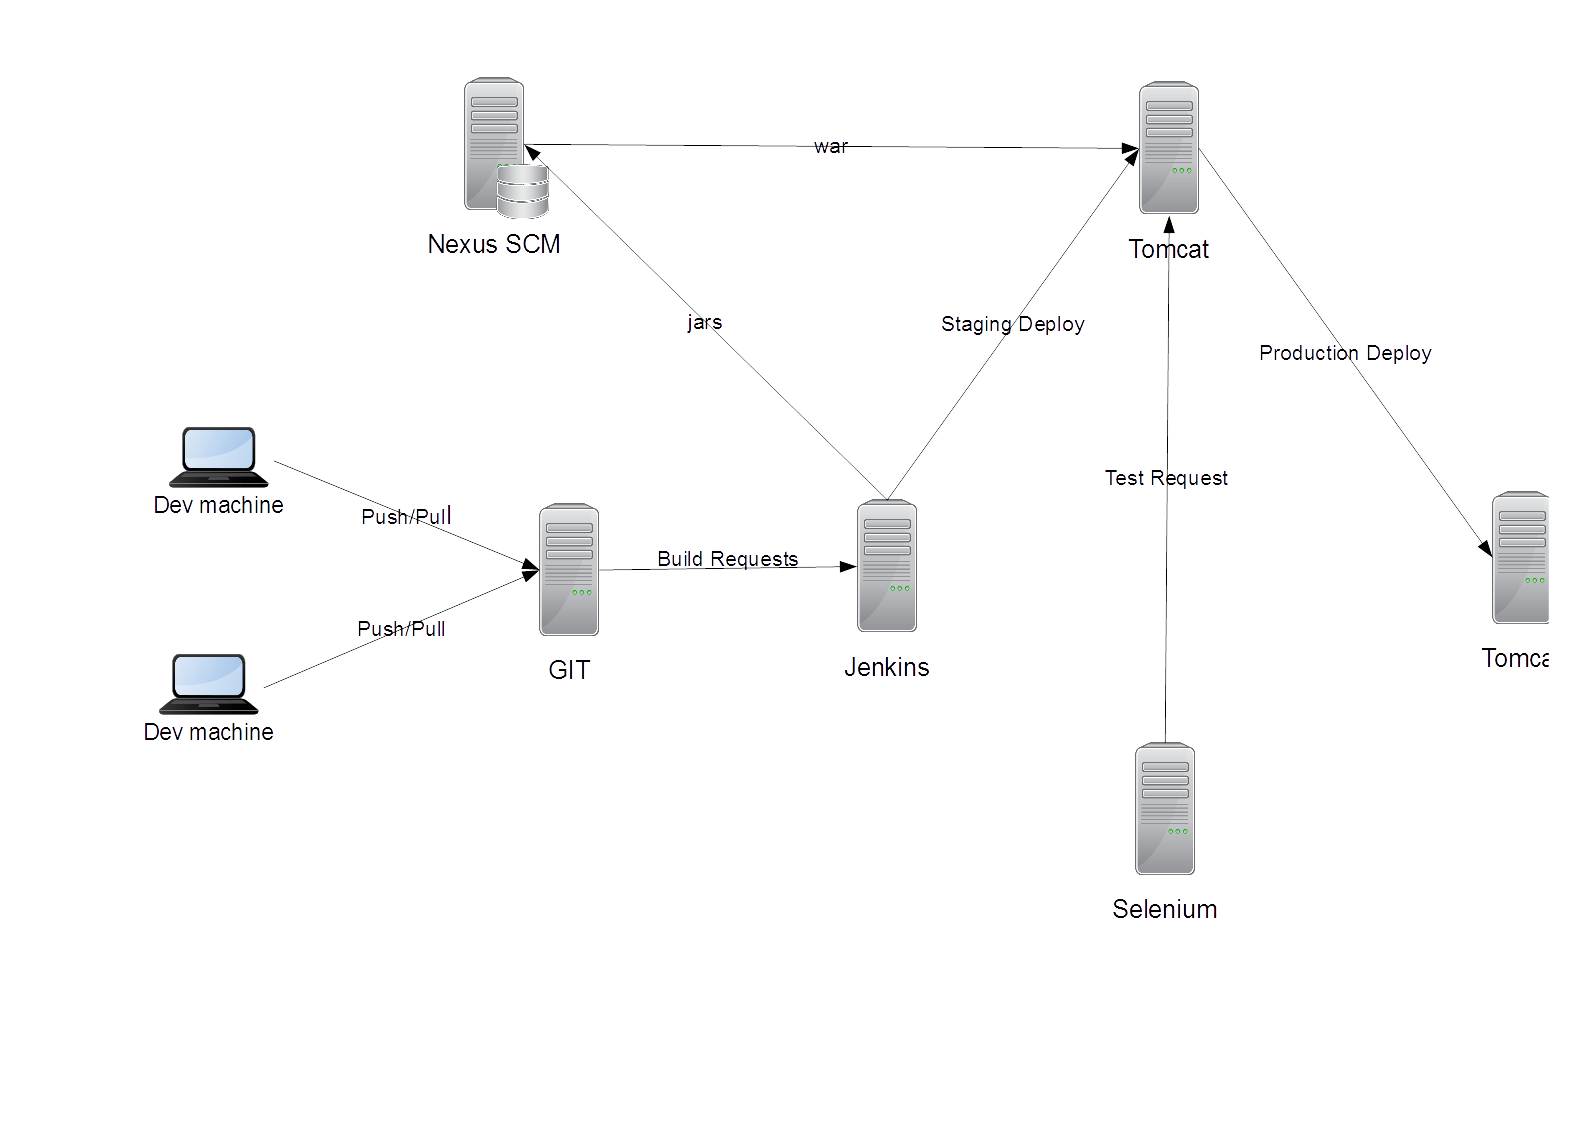
\epsfig{width=6in, file=pipeline.png}
\caption{C.I Pipeline}
\end{center}

\end{figure}
\pagebreak
\section{SEQUENCE DIAGRAM}
\par A Sequence diagram is an interaction diagram that shows how processes operate with
one another and in what order. It is a construct of a Message Sequence Chart. A sequence
diagram shows object interactions arranged in time sequence. It depicts the objects and classes
involved in the scenario and the sequence of messages exchanged between the objects needed
to carry out the functionality of the scenario.
\begin{figure}[h]
\begin{center}

\hspace{.0 in}
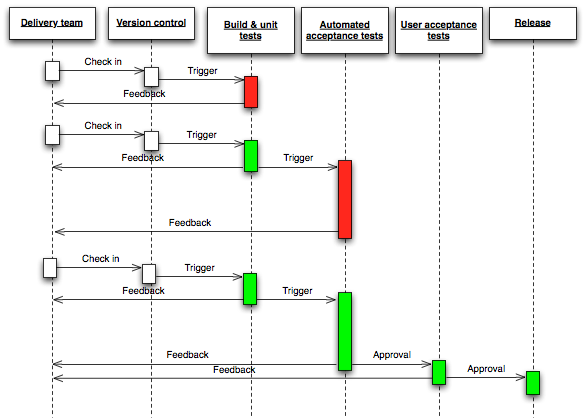
\epsfig{width=6in, file=sequence.png}
\caption{Sequence}
\end{center}

\end{figure}
\par
The input to the pipeline is a particular revision in version control. Every change creates a build that will, rather like some mythical hero, pass through a sequence of tests of, and challenges to, its viability as a production release. This process of a sequence of test stages, each evaluating the build from a different perspective, is begun with every commit to the version control system, in the same way as the initiation of a continuous integration process.
\par
As the build passes each test of its fitness, confidence in it increases. Therefore, the resources that we are willing to expend on it increase, which means that the environments the build passes through become progressively more production-like. The objective is to eliminate unfit release candidates as early in the process as we can and get feedback on the root cause of failure to the team as rapidly as possible. To this end, any build that fails a stage in the process will not generally be promoted to the next.
\chapter{IMPLEMENTATION}
Implementation is the stage in the project where the theoretical design is turned into a working system and is giving confidence about the new system to users that it will work effectively. It involves careful planning, investigation of the current system and it constraints on implementation, design of achieve the changeover, an evolution of change over method.

\section{LANGUAGES AND PLATFORM USED}
\par Continuous integration (CI) is an integral part of an agile software development setup. Sprint after sprint, teams strive to "not break the build" while delivering incremental features. But when developers focus completely on adding features, code errors can sometimes creep in and render the software unusable. To stop such errors from being integrated into the software configuration management (SCM), a CI server is the gatekeeper that helps keep a tab on code quality. Even if the code is integrated to SCM, a CI server can quickly tell you what went wrong
\par
	The platforms and softwares that are used in the continuous integration pipeline implementation is mentioned below 
\subsection{GitHub}
\par GitHub is a web-based Git or version control repository and Internet hosting service. It offers all of the distributed version control and source code management (SCM) functionality of Git as well as adding its own features. It provides access control and several collaboration features such as bug tracking, feature requests, task management, and wikis for every project.
\par
GitHub offers both plans for private and free repositories on the same account which are commonly used to host open-source software projects. 
\subsection{Amazon Web Services (AWS)}
\par Amazon Web Services (AWS), a subsidiary of Amazon.com, offers a suite of cloud-computing services that make up an on-demand computing platform. These services operate from 16 geographical regions across the world. They include Amazon Elastic Compute Cloud, also known as "EC2", and Amazon Simple Storage Service, also known as "S3". As of 2016 AWS has more than 70 services, spanning a wide range, including compute, storage, networking, database, analytics, application services, deployment, management, mobile, developer tools and tools for the Internet of things. Amazon markets AWS as a service to provide large computing capacity quicker and cheaper than a client company building an actual physical server farm.\\
\subsection{Jenkins}
\par Jenkins helps to automate the non-human part of the whole software development process, with now common things like continuous integration, but by further empowering teams to implement the technical part of a Continuous Delivery. It is a server-based system running in a servlet container such as Apache Tomcat. It supports SCM tools including AccuRev, CVS, Subversion, Git, Mercurial, Perforce, Clearcase and RTC, and can execute Apache Ant, Apache Maven and sbt based projects as well as arbitrary shell scripts and Windows batch commands. The creator of Jenkins is Kohsuke Kawaguchi. Released under the MIT License, Jenkins is free software.
\par
Builds can be triggered by various means, for example by commit in a version control system, by scheduling via a cron-like mechanism and by requesting a specific build URL. It can also be triggered after the other builds in the queue have completed.
\par

Jenkins functionality can be extended with plugins.\\
\subsection{Apache Maven}
Maven is a build automation tool used primarily for Java projects. The word maven means "accumulator of knowledge" in Yiddish.
\par
Maven addresses two aspects of building software: first, it describes how software is built, and second, it describes its dependencies. Contrary to preceding tools like Apache Ant, it uses conventions for the build procedure, and only exceptions need to be written down. An XML file describes the software project being built, its dependencies on other external modules and components, the build order, directories, and required plug-ins. It comes with pre-defined targets for performing certain well-defined tasks such as compilation of code and its packaging.
\par
Maven dynamically downloads Java libraries and Maven plug-ins from one or more repositories such as the Maven 2 Central Repository, and stores them in a local cache.This local cache of downloaded artifacts can also be updated with artifacts created by local projects. Public repositories can also be updated.
\par
Maven can also be used to build and manage projects written in C\#, Ruby, Scala, and other languages. The Maven project is hosted by the Apache Software Foundation, where it was formerly part of the Jakarta Project.
\subsection{FindBugs}
\par
FindBugs is an open source static code analyser created by Bill Pugh and David Hovemeyer which detects possible bugs in Java programs. Potential errors are classified in four ranks: (i) scariest, (ii) scary,   (iii) troubling and (iv) of concern. This is a hint to the developer about their possible impact or severity.FindBugs operates on Java bytecode, rather than source code. The software is distributed as a stand-alone GUI application
\subsection{Jacoco}
\par
Jacoco is a free code coverage library for Java. 
I use it because it is very simple to add to all types of build including ANT and Maven, and it is also very simple to add to Java containers or a standalone JVM.
\subsection{Apache Tomcat}
\par
Apache Tomcat, often referred to as Tomcat Server, is an open-source Java Servlet Container developed by the Apache Software Foundation (ASF). Tomcat implements several Java EE specifications including Java Servlet, JavaServer Pages (JSP), Java EL, and WebSocket, and provides a "pure Java" HTTP web server environment in which Java code can run.

Tomcat is developed and maintained by an open community of developers under the auspices of the Apache Software Foundation, released under the Apache License 2.0 license, and is open-source software.
\subsection{Heroku}
\par
Heroku is a cloud Platform-as-a-Service (PaaS) supporting several programming languages that is used as a web application deployment model. Heroku, one of the first cloud platforms, has been in development since June 2007, when it supported only the Ruby programming language, but now supports Java, Node.js, Scala, Clojure, Python, PHP, and Go. For this reason, Heroku is said to be a polyglot platform as it lets the developer build, run and scale applications in a similar manner across all the languages. Heroku was acquired by Salesforce.com in 2010.
\subsection{New Relic APM}
\par
Lew Cirne founded New Relic in 2008 with a revolutionary vision: To deliver application performance monitoring (APM) as a purely SaaS product. By embracing the power and accessibility of the cloud, New Relic grew rapidly and quickly became an integral tool for developers, IT ops teams, and executives around the world.

\subsection{Node.js}
\par
Node.js is an open-source, cross-platform JavaScript runtime environment for developing a diverse variety of server tools and applications. Although Node.js is not a JavaScript framework,many of its basic modules are written in JavaScript, and developers can write new modules in JavaScript. The runtime environment interprets JavaScript using Google's V8 JavaScript engine.

Node.js has an event-driven architecture capable of asynchronous I/O. These design choices aim to optimize throughput and scalability in Web applications with many input/output operations, as well as for real-time Web applications.

\subsection{AngularJS}
\par
Node.js is an open-source, cross-platform JavaScript runtime environment for developing a diverse variety of server tools and applications. Although Node.js is not a JavaScript framework,many of its basic modules are written in JavaScript, and developers can write new modules in JavaScript. The runtime environment interprets JavaScript using Google's V8 JavaScript engine.

Node.js has an event-driven architecture capable of asynchronous I/O. These design choices aim to optimize throughput and scalability in Web applications with many input/output operations, as well as for real-time Web applications.
\pagebreak
\section{HOW IT IS IMPLEMENTED}
\par For demonstration, a Calculator application was developed in traditional and in C.I manner. The sample calculator is developed in Java, NodeJs, AngularJs.
Initially the modules of the sample calculator app has been developed in java individually and integrated them manually, It was really time consuming and ambiguous. Then apply the concept of version control.
\par
   For version control, Created a Repository named LogicBaker in Git-Hub and cloned to individual systems. Created modules given to each member in java After Coding the individual modules the team members commit to Git-Hub, irrespective on the platform which each one has build.
   
   \par
   The integration is much helpful via version controlling.  But to modify the existing code pushed by other individual member, it was time consuming. Because there was no standardization in the module codes. To standardize the project we mavenized the project thus the project had a standard and the reusing libraries  occur only a single copy in the entire project provided an active Internet connection is required for at the time of cloning and first build. \par
   The main advantages of the using a Continuous Integration is deploying the currently developed modules in the private online space. Thus every member of the project can view the project and suggests the changes via notifying the developer thus it is helpful to the developers. \par
   We use jenkins as C.I handler, Jenkins is an open source automation server written in Java. The project was forked from Hudson after a dispute with Oracle. It is a server-based system running in a servlet container such as Apache Tomcat. Jenkins provide a automation platform which each module can be integrated and build and error can be notified to entire personal participating in project development.
   \par For unit testing while developing the Test automation is added i jenkins. The test Automation plugin is added to Jenkins depending upon the nature of the development process dealing with. Which involve programming framework, language etc. Since we use Java , we use find-bugs and Check style in Jenkins.. Also added Jacoco , For code coverage
 \par
  For much more flexibility the entire CI process can be handled by Heroku. Heroku is a cloud Platform-as-a-Service (PaaS) supporting several programming languages that is used as a web application deployment model. Heroku, one of the first cloud platforms. \par
  The same mavenised java application is pushed to Heroku Git hub. Also code the same application in Node.js for efficient viewing, and deployed in Heroku server. \par
  New Relic plugin is added to the Calc Application(Node.Js). Its an application performance manager. It tracks real time response time and throughput.
   \par
   Compared the various CI development process using the testing calculator application and founded its much better than the traditional development process. The finding are noted and submitted to the Tech11 company and found much decrease in their development time and cost.
    \newpage

\section{SCREEN SHOTS}
\subsection{GitHub}
\begin{itemize}
\item \par A developer can change the program files locally and commit the changes to the remote GitHub repository using this GitHub desktop application. The changes will be automatically send to the CI server.
\begin{figure}[h]
\begin{center}
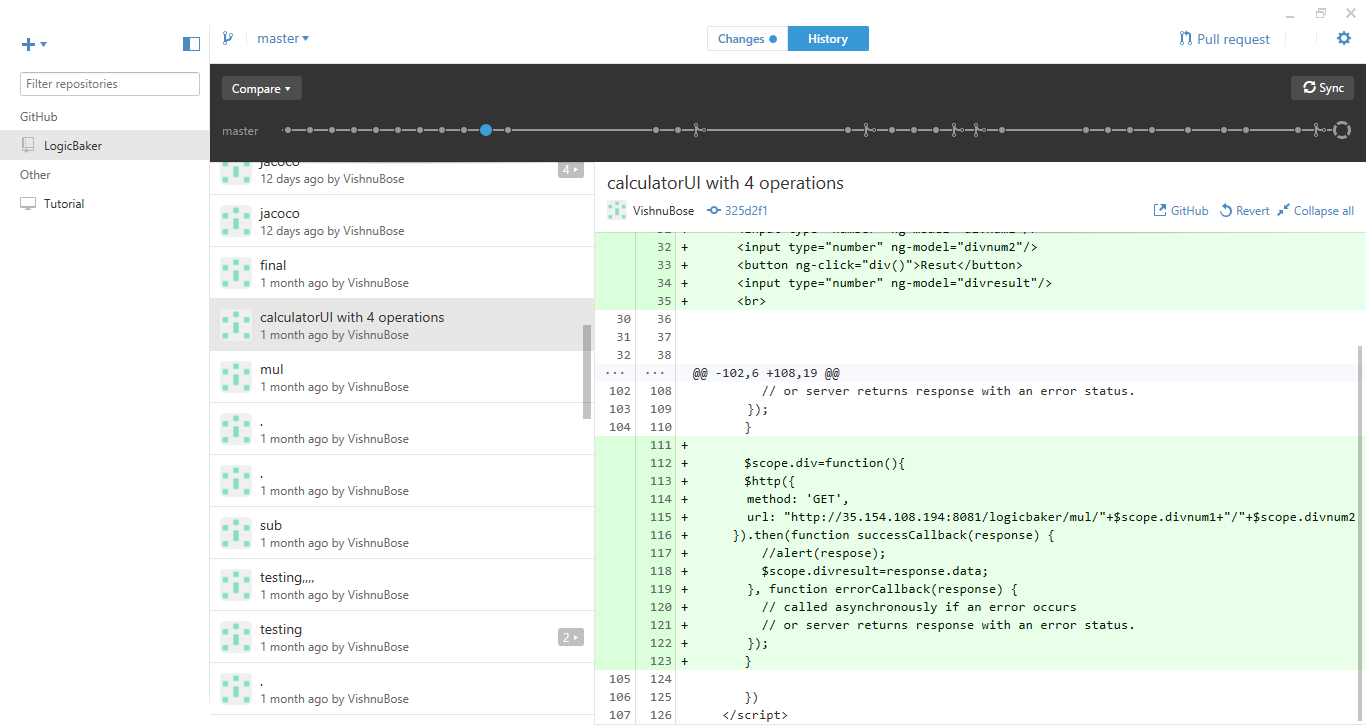
\includegraphics[scale=.47]{git.png}
\caption{GitHub GUI in windows}
\label{GitHub GUI in windows}
\end{center}
\end{figure}
\pagebreak
\begin{figure}[h]
\begin{center}
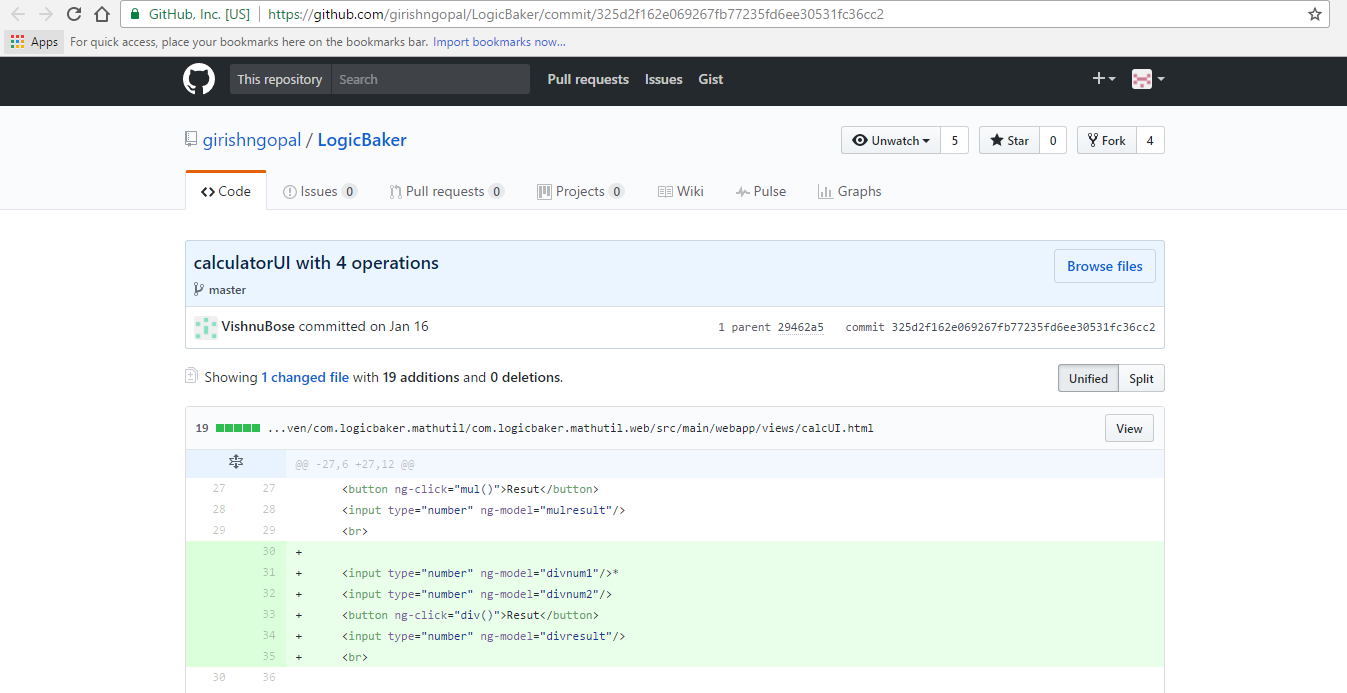
\includegraphics[scale=.47]{remote.png}
\caption{GitHub remote repository }
\label{GitHub remote repository}
\end{center}
\end{figure}
\end{itemize}
\pagebreak
\newpage
\subsection{Amazon Web Services (AWS)}
\begin{itemize}
\item \par AWS is a IaaS (Infrastructure as a Service).
Here Jenkins is Working on Ubuntu installed in aws 
\begin{figure}[h]
\begin{center}
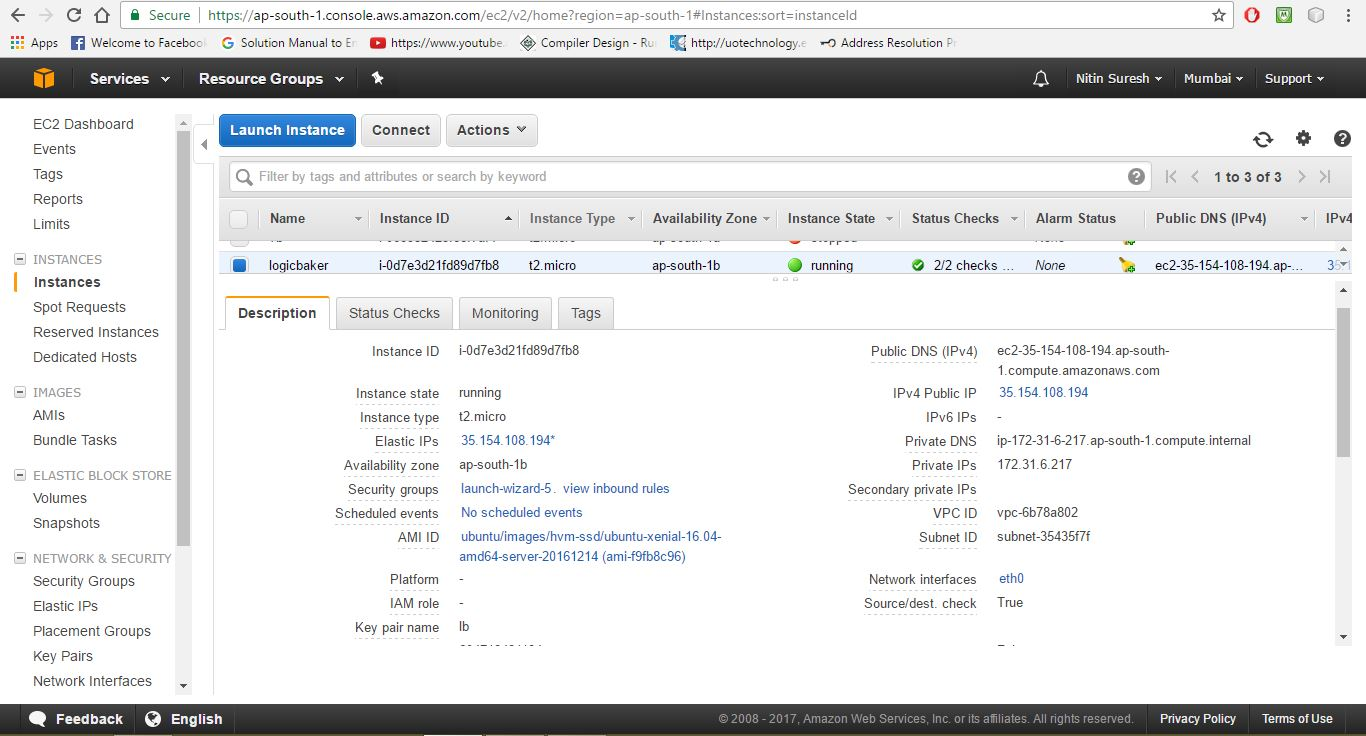
\includegraphics[scale=.47]{aws.png}
\caption{Amazon Web Services Dashboard}
\label{Amazon Web Services Dashboard}
\end{center}
\end{figure}
\end{itemize}
\pagebreak
\newpage
\subsection{Jenkins}
\begin{itemize}

\item \par Whenever a change occurred in the GitHub the change will be automatically push into the ci server ie, Jenkins.It is then builded and ready to deploy
\begin{figure}[h]
\begin{center}
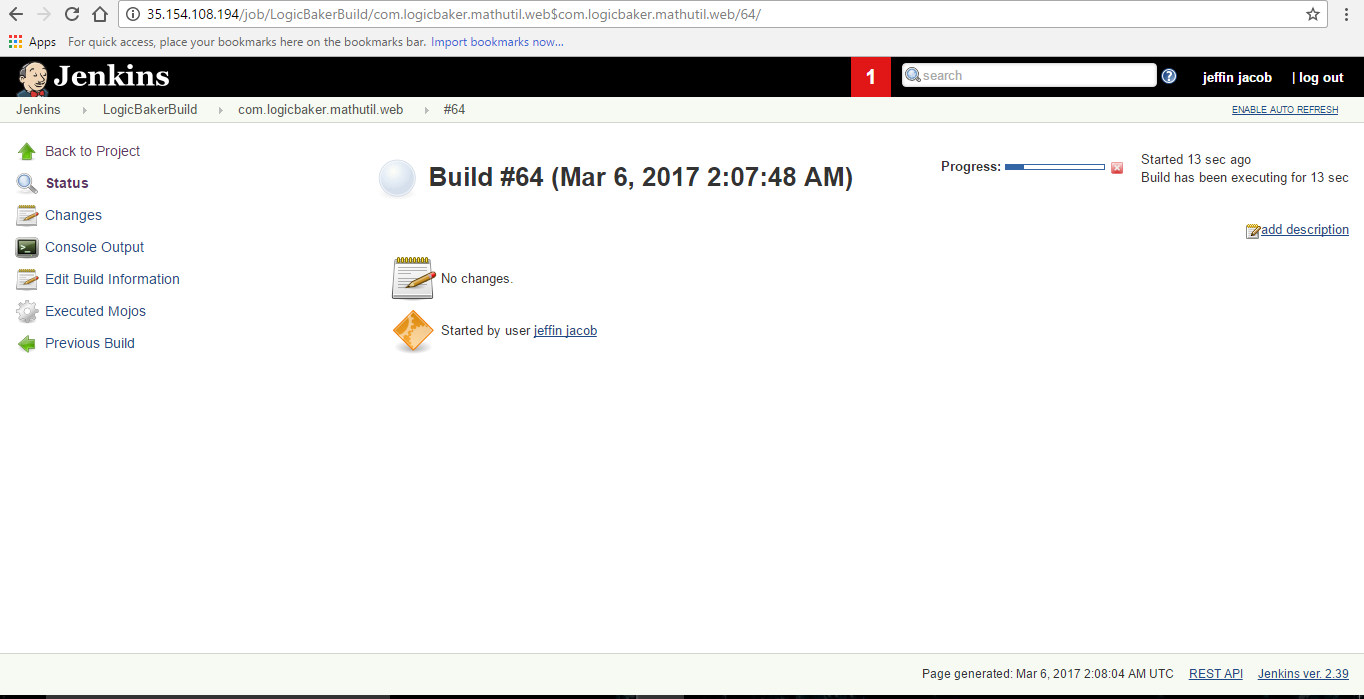
\includegraphics[scale=.47]{jnks.png}
\caption{Jenkins dashboard building calculator app}
\label{Jenkins dashboard building calculator app}
\end{center}
\end{figure}
\item \par We can configure the deployment with FindBugs or Jacoco as per the requirement
\newpage
\subsection{Calculator app in Jenkins}
\item \par Calculator application deployed automatically by Jenkins
\begin{figure}[h]
\begin{center}
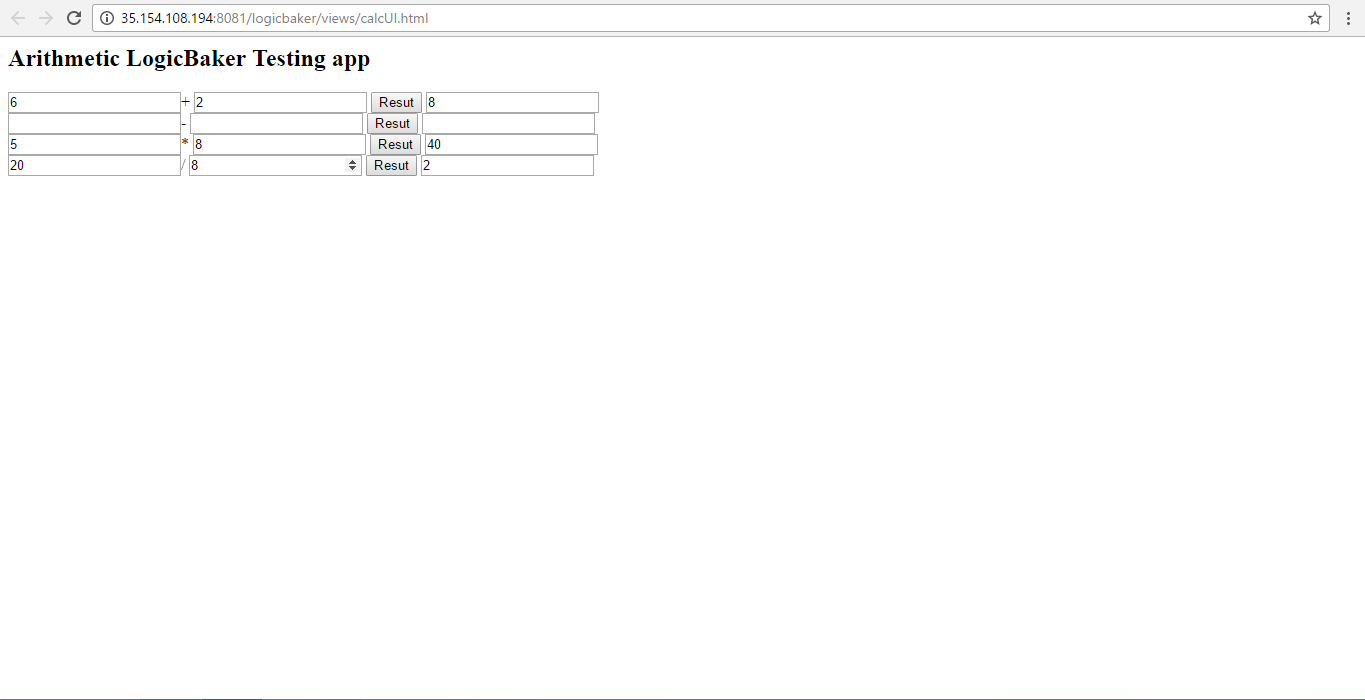
\includegraphics[scale=.47]{app.png}
\caption{Calculator app in Jenkins}
\label{Calculator app in Jenkins }
\end{center}
\end{figure}
\end{itemize}
\newpage
\subsection{Heroku}
\begin{itemize}
\item \par The same application is deployed using another pipeline Heroku. Heroku is a PaaS (Platform as a Service) here platforms for each language is available,complexity of an IaaS is reduced in Heroku
\begin{figure}[h]
\begin{center}
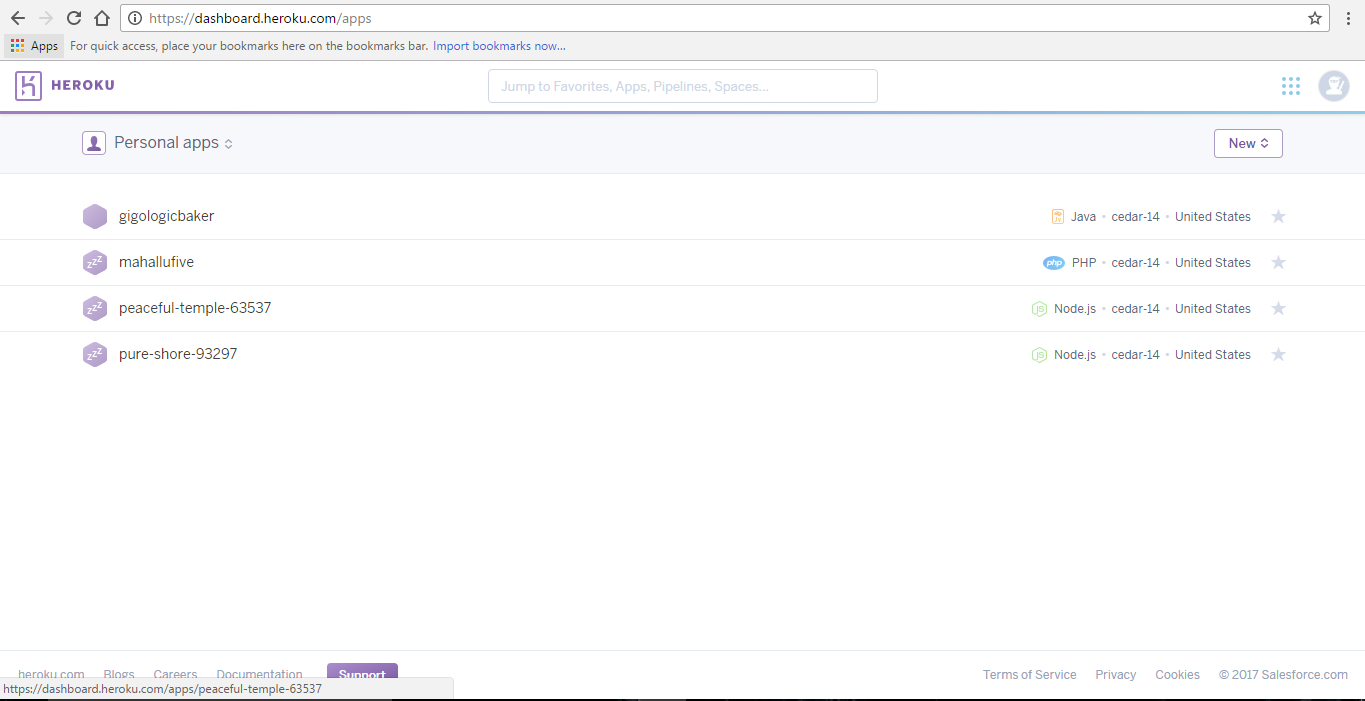
\includegraphics[scale=.47]{hrk.png}
\caption{Heroku Dashboard}
\label{Heroku Dashboard}
\end{center}
\end{figure}
\end{itemize}
\newpage
\subsection{Calculator app in Heroku}
\begin{itemize}
\item \par Calculator application deployed automatically by Heroku
\begin{figure}[h]
\begin{center}
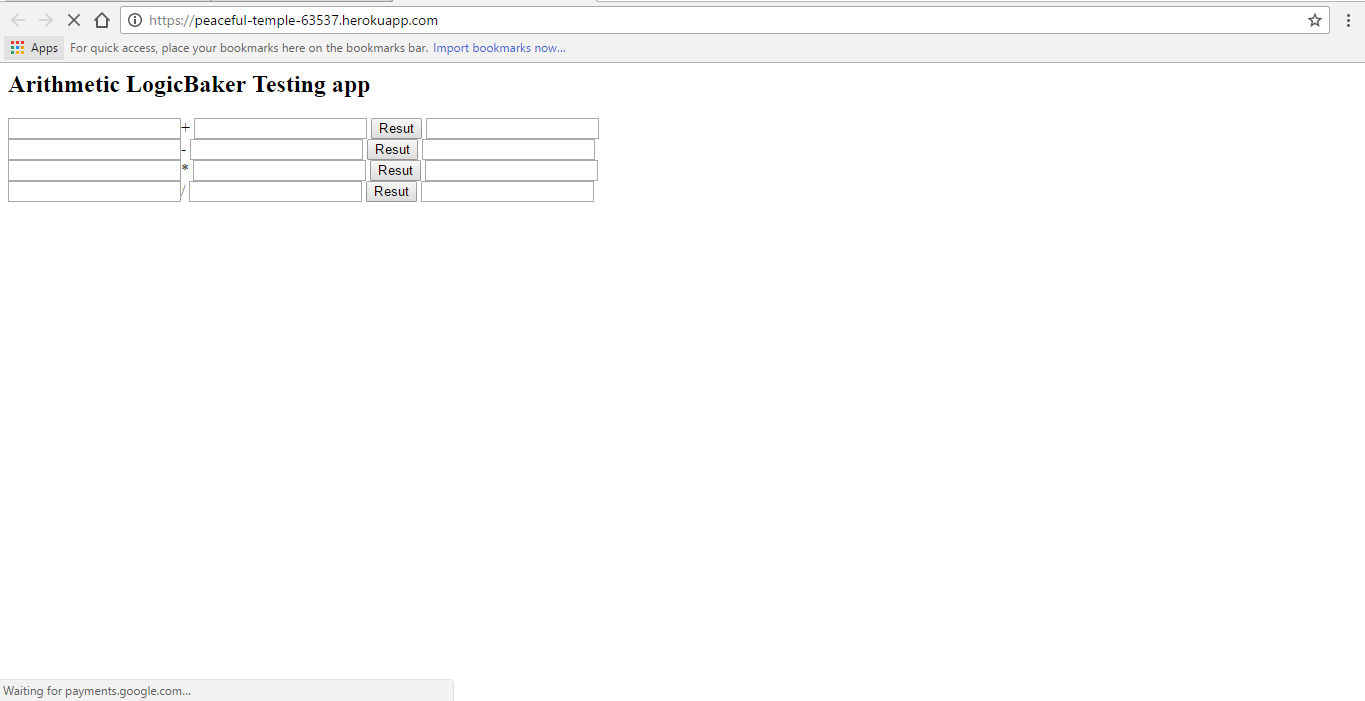
\includegraphics[scale=.47]{app1.png}
\caption{Calculator app in Heroku}
\label{Calculator app in Heroku}
\end{center}
\end{figure}
\end{itemize}
\newpage
\subsection{New Relic Monitoring}
\begin{itemize}
\item \par The deployed app can be monitored using the new Relic APM.
\begin{figure}[h]
\begin{center}
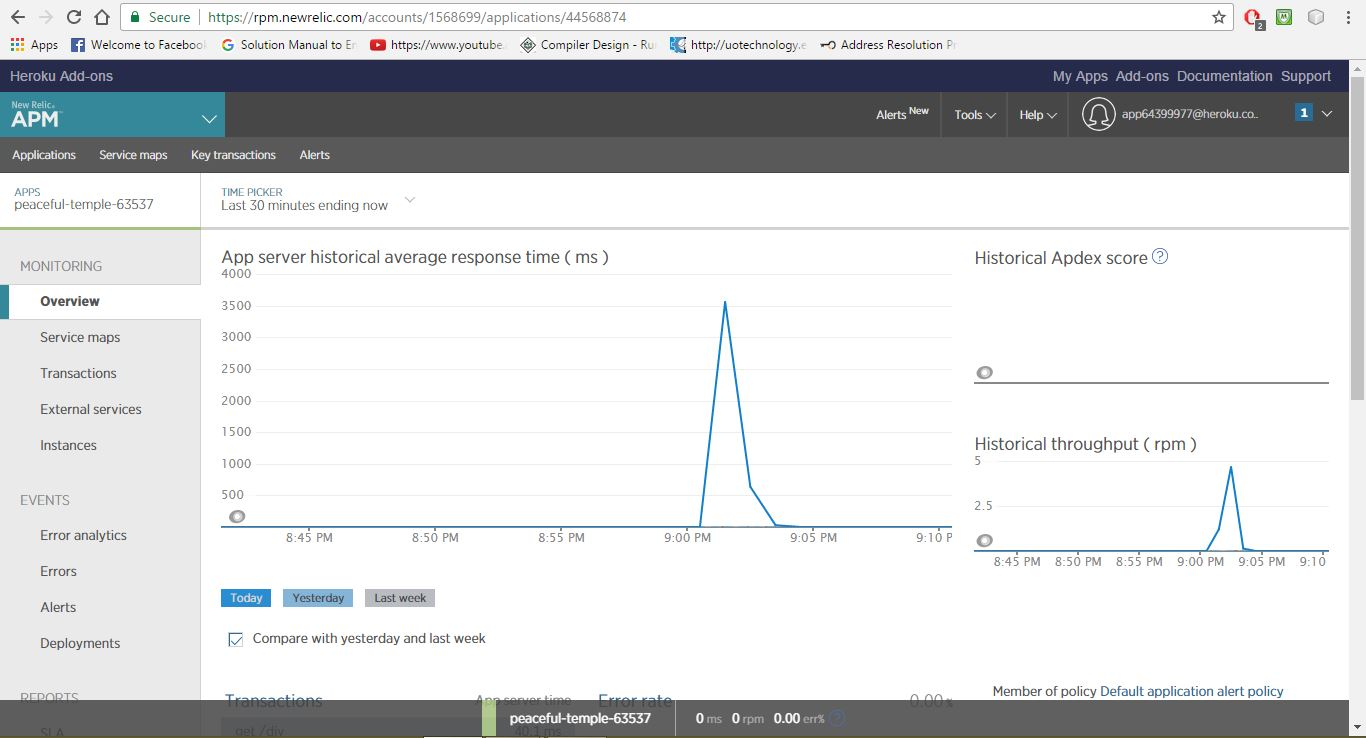
\includegraphics[scale=.47]{newrelic.png}
\caption{New Relic APM monitoring}
\label{New Relic APM monitoring}
\end{center}
\end{figure}
\end{itemize}
\newpage

\newpage
\chapter{TESTING}
\par When a system is developed, it is hoped that it performs properly. In practice, however some errors always occur. The main purpose of testing an information system is to find the error and correct them. A successful test is one that finds an error. System testing is a critical aspect of Software Quality Assurance and represents the ultimate review of specification, design and coding. Testing is the process of executing a program with the intent of finding an as yet undiscovered error. Nothing is complete without testing. Testing is vital to the success of the system.\\
\par The main objectives of the system testing are:\\
\begin{itemize}
\item To ensure during operation the system will perform as per specification. 
\item To make sure that the system meets user requirements during operation.
\item To verify that the controls incorporated in the system function as intended.
\end{itemize}
\par If the testing conducted successfully, it will uncover errors in the software. As a secondary benefit, testing demonstrates that the software functions appear to be working according to specification and that performance requirements appear to have been satisfied.\\
\par The system “Save Me” is tested in such a way that almost all errors that may occur are found and corrected. The test process carried out in this system includes the following:\\
\section{CODE TESTING}
\par In code testing the logic of the developed system is tested. For this every module of the program is executed to find any error. To perform specification test, the examination of the specifications stating what the program should do and how it should perform under various conditions.This testing was done side by side with coding. This examines the logic of the program. In Java special test cases are used for testing the code. Every part of the program was tested in this phase.

\section{UNIT TESTING}
\par Unit testing is undertaken after a module has been coded and reviewed. Before carrying this testing, the unit test cases have to be designed and the test environment for the unit under test has to be developed. The various test cases are driver and stub modules. The main objective is to determine the correct working of the individual modules. During the testing each module is isolated from other modules and individually unit tested. It involves a precise definition of the test cases, testing criteria, and management of test cases. The modules that are tested include \\
Android module, Server module and Sensing module.

\section{INTEGRATION TESTING}
\par System testing does not test the software as a whole, but rather than integration of each module in the system. The primary concern is the compatibility of individual modules. One has to find areas where modules have been designed with different specifications of data lengths, type and data element name. Testing and validation are the most important steps after the implementation of the developed system. The system testing is performed to ensure that there are no errors in the implemented system. The software must be executed several times in order to find out the errors in the different modules of the system. Each of the modules were integrated together and subjected to testing. \\
\section{VALIDATION TESTING}
\par Validation refers to the process of using the new software for the developed system in a live environment i.e., new software inside the organization, in order to find out the errors. The validation phase reveals the failures and the bugs in the developed system. It will come to know about the practical difficulties the system faces when operated in the true environment. Validation test was performed in the Login section. By testing the code of the implemented software, the logic of the program can be examined. A specification test is performed to check whether the specifications stating the program are performing under various conditions. Apart from these tests, there are some special tests conducted which are given below:
\begin{itemize}
\item Peak load test This determines whether the new system will handle the volume of activities when the system is at the peak of its processing demand. The test has revealed that the new system is capable of handling the demands at the peak time.
\item Storage testing This determines the capacity of the new system to store transaction data on a disk or on other files. The proposed software has the required storage space
available.
\item Performance time testing This test determines the length of the time used by the system to process transaction data.
\end{itemize}
\section{SYSTEM TESTING}
\par After all units of a program have been integrated together and tested, system testing is taken up. It is same for both procedural and object oriented programming. System tests are designed to validate a fully developed system to assure that it meets its requirements. The system test cases can be classified into performance and functionality test cases. The functionality test cases are designed to check whether the software satisfies the functional requirements as documented in the SRS document. The performance tests on the other hand test the conformance of the system with non-functional requirements of the system.\\
\section{OUTPUT TESTING}
\par After the performance of unit testing, the next step is output testing. No system would be useful if it does not produce the required output in the specific format, thus output format on the screen is found to be correct when the format was designed in the system phase according to the user need.\\
\par The maintenance of software is the time period in which software product performs useful works. Maintenance activities involve making enhancement to software product, adapting product to new environment and correcting problems. It includes both the improvement of the system function.
\par It may involve the continuing involvement of a large proportion of computer department resources. The main task may be to adapt existing system in a changing environment. System should not be changed casually following informal requests. To avoid unauthorized amendments, all requests for change should be channeled to a person nominated by management. The nominated person has sufficient knowledge of the organizations computer based systems to be able to judge the relevance of each proposed change.
\par No annual costs for support or maintenance are required. Of course, the individual system components come with limited warranty from the manufacturers, eg:, the PC, mobile phones, etc.
\par There is no obligation to purchase or pay for any extended maintenance or support.
\section{GOAL OF TESTING}
\par Many users may use our project. So the project designer must test all the modules of the project. The main goal of our project is, whenever user uses our project, it should run without any error.
\section{PASS/FAIL CRITERIA}
The pass/fail criteria specifies a set of constraints whose satisfaction leads to approval or disapproval of the proper functioning of the system .
\section{PASS CRITERIA}
\par The system must meet all the functional and non-functional requirements. Pass all the test cases, get the expected response, and get acceptable performance to be tested pass.
\begin{itemize}
\item	Developer can commit and push.
\item	Successful build
\item	Positive feedback
\end{itemize}
\section{FAIL CRITERIA}
\par If one of the following situations happens, the system is considered to fail:
\begin{itemize}
\item	Conflict
\item   Build failure
\item	Negative feedback
\end{itemize}
\pagebreak
\section{TEST REPORTS}
The detailed test reports prepared for each function. A sample test report is given below:
\begin{table}[!htb]
\centering
\caption{Test Report}
\label{Test Report}
\begin{tabular}{|l|l|}
\hline
Name                                                                                & Continuous Integration Pipeline Implementation for Tech11Software                                               \\ \hline
Version                                                                             & 1.0                                                                  \\ \hline
Author                                                                              & Aswin G Sugunan, Jeffin Jacob, Nitin Suresh,Vishnu Bose.              \\ \hline
Approved By                                                                         & Self                                                                 \\ \hline
Date                                                                                & \today                                            \\ \hline
Role                                                                                & Developer can operate the system.                                          \\ \hline
Prerequisite                                                                        & The Developer is logged into the system by the repository administrator                                   \\ \hline
Developer/Actor                                                                          & System Response                                                      \\ \hline
Run Applications                                                                    & Developer can continuously integrate and there always a ready-to deploy build. \\ \hline
Handle developer Data                                                                    &The server can handle various developer data                                                                      \\ \hline
                                                                                    
\begin{tabular}
[c]{@{}l@{}}The test project\\ was successfully\\ saved
\end{tabular} 
&                                                                      \\ \hline
\end{tabular}
\end{table}
\par Test case preparation helps the user and the developer to find and fix the errors easily and in advance. Save Me is well tested with the proper test cases and thus passed a better unit test. Elaborated test cases also prepared subjected the system for thorough testing. The test cases prepared are in the above format.

\chapter{FUTURE SCOPE}
\par CI was created with the goal of eliminating the old “big bang integration” practices in which software modules are developed in isolation and integration is postponed until the end of the project - and quite frequently the timing and project cost of the final integration work is deeply underestimated. In order to eradicate this hindrance, many agile development experts have now converted integration into a continuous process. When integrations are performed on a daily basis, the final, uncontrolled big-bang integration will vanish from the modern development process.

The CI process is now a daily practice of software developers worldwide, and an important reason why other best practices such us automated testing have become mainstream throughout the software industry.


\chapter{CONCLUSION}
\par 
Putting software into production is slow and risky. Optimizing this process has the potential to make software development overall more effective and efficient. Continuous Delivery might therefore be one of the best options to improve software projects.
\par
Moving to Continuous Deployment will change the development dramatically. It will make the development more productive and lead to a more stable and better product.
\par
Continuous Delivery aims at regular, reproducible processes to deliver software much like Continuous Integration does to integrate all changes. While Continuous Delivery seems like a great option to decrease time to market it actually has much more to offer: It is an approach to minimizing risk in a software development project because it ensures that software can actually be deployed and run in production. So any project can gain some advantage even if it is not in a very competitive market where time to market is not that important after all.
\renewcommand{\bibname}{\uppercase{REFERENCES}}
\begin{thebibliography}{999}
\addcontentsline{toc}{chapter}{\hspace{0.5cm} REFERENCES}
\raggedright
\bibitem{r1} Duvall, Paul, Steve Matyas, and Andrew
Glover, \quotes{Continuous Integration: Improving Software Quality and Reducing Risk}, \textit{ Addison Wesley, Boston} 2007
\bibitem{r1}Ade Miller , \quotes{ A Hundread Days Of Continuous Integration }, \textit{ Agile 2008 Conference} 2008.

\bibitem{r1}Miller, Ade and Eric Carter , \quotes{Agility and the
Inconceivably Large.}, \textit{ Agile 2007 Conference} 
13-17 Aug,
Washington DC, 2007. 
\bibitem{r1}Kniberg, Henrik. , \quotes{Scrum and XP from the
Trenches: How we do Scrum.}, \textit{  C4Media Inc.} 
, 2007. 
\bibitem{r1} Magennis, Troy, \quotes{Continuous Integration and Automated Builds at Enterprise Scale}, \textit{ Online posting} 2007, \hspace{2pt}  \url{ http://aspiringtechnology.com/blogs/troym/archive/2007/11/26/Does ContinuousIntegrationScale.aspx}
\bibitem{r2}The Zend Blueprint for Continuous Delivery, Zend Technologies, \url{www.zend.com/continuousdelivery.}
\bibitem{r3} Adopting the IBM DevOps approach for
continuous software delivery, \hspace{2pt}
 \url{http://www.ibm.com/developerworks/libr
ary/d-adoption-paths/}.

\bibitem{r3}Understanding DevOPs-Infrastructure as a code,\hspace{2pt}
 \url{https://sdarchitect.wordpress.com/2012/12
/13/infrastructure-as-code/}.
\bibitem{r1} DevOps Distilled, The Three underlying principles, \url{ http://www.ibm.com/developerworks/libr ary/se-devops/part1/ }. 
\bibitem{r2}DevOps for Dummies – by Sanjeev Sharma, \url{https://www14.software.ibm.com/webapp/ iwm/web/signup.do?source=swg-rtl-sdwp&S_PKG=ov18162}.
\bibitem{r1}Continuous Integration, \url{http://www.ccpace.com/asset_files/Continuous_Intergration}.
\end{thebibliography}
\chapter*{GLOSSARY}
\addcontentsline{toc}{chapter}{\hspace{0.5cm} GLOSSARY}
\rhead{\empty}
%\begin{center}

\textbf{DFD}  : Data Flow Diagram
\par \textbf{CI} : Continuous Integration
 \par \textbf{AWS} : Amazon Web Services
\par \textbf{APM} : Application Performance Monitoring
\par  \textbf{SCM} : Software configuration Management
\par \textbf{IaaS} : Infrastructure as a Service
\par \textbf{PaaS} : Platform as a Service
\par \textbf{JVM} : Java Virtual Machine
\newpage
\chapter*{APPENDIX I}
\renewcommand{\bibname}{\uppercase{APPENDIX I}}
%\begin{thebibliography}{999}
\addcontentsline{toc}{chapter}{\hspace{0.5cm} APPENDIX I}
%\chapter{APPENDIX 1}
\large{\textbf{\text{SAMPLE TESTING CODE}}}
\appendix

\textbf{Adder.java}
\begin{lstlisting}
package com.logicbaker.mathutil.adder;

public class Adder {
	
	public int add(int number1,int number2){
		return number1+number2;
	}

}



\end{lstlisting}

%\underline{Calculator modules (without mavenization)}

\textbf{Subtract.java}
\begin{lstlisting}
package com.logicbaker.mathutil.adder;

public class Subtract {
	
	public static int subtratc(int number1,int number2){
		return number1-number2;
	}

}



\end{lstlisting}


\textbf{Multiply.java}
\begin{lstlisting}
package com.logicbaker.mathutil;

public class Multiply {
	
	public static int multiply(int number1,int number2){
		return number1*number2;
	}

}




\end{lstlisting}


\textbf{Divider.java}
\begin{lstlisting}
package com.logicbaker.mathutil;

public class Divider {
	
	public static int divider(int number1,int number2){
		return number1/number2;
	}
	

}




\end{lstlisting}


\textbf{Calculator.java}
\begin{lstlisting}
package com.logicbaker.mathutil.calculator;

import org.apache.commons.math3.analysis.function.Abs;

import com.logicbaker.mathutil.Adder;


public class Calculator {
	
  public static void main(String args[]){
	  Abs abs = new Abs();
	  System.out.println(abs.value(1.00));
	  
	  Adder adder = new Adder();
	  System.out.println(adder.add(1, 2));
	  
  }
  
  

}





\end{lstlisting}


\textbf{pom.XML}
\begin{lstlisting}
<?xml version="1.0" encoding="UTF-8"?>

-<project xsi:schemaLocation="http://maven.apache
.org/POM/4.0.0 http://maven.apache.org/xsd
/maven-4.0.0.xsd">-

<modelVersion>4.0.0</modelVersion>

<groupId>com.logicbaker.mathutil</groupId>

<artifactId>com.logicbaker.mathutil</artifactId>

<version>0.0.1-SNAPSHOT</version>

<packaging>pom</packaging>


-<modules>

<module>com.logicbaker.mathutil.adder</module>

<module>com.logicbaker.mathutil.Calc</module>

<module>com.logicbaker.mathutil.substract</module>

<module>com.logicbaker.mathutil.multiply</module>

<module>com.logicbaker.mathutil.divide</module>

<module>com.logicbaker.mathutil.web</module>

</modules>

</project>




\end{lstlisting}

\newpage
%\chapter{APPENDIX 1}

\begin{theindex}

\addcontentsline{toc}{chapter}{\hspace{0.5cm} INDEX}
\rhead{\empty}
\lhead{\empty}
\lfoot{\empty}
%\hspace{.1in}
\vspace{.2in}
\large\textbf{A}
\item  Amazon Web Services 22, 28
\item  AngularJS , 25
\item Apache Tomcat  , 24
\item Artifact Manager , 11
\vspace{.2in}

\large\textbf{C}
\item Conclusion , 41
\item  Continuous Integration Handler , 12
\item Continouos Deployment , 13
\vspace{.2in}

\large\textbf{D}
\item Data Flow Diagram , 15
\vspace{.2in}

\large\textbf{F}
\item Flow Diagram , 17
\vspace{.2in}

\large\textbf{G}
\item Gantt chart , 7
\item Goal of testing, 37
\vspace{.2in}

\large\textbf{H}
\item Heroku , 24,31
\vspace{.2in}

\large\textbf{I}
\item Introduction , 1
\item Integration Testing , 35

\vspace{.2in}
\large\textbf{J}
\item Jenkins , 22,29
\item Jacoco , 24
\vspace{.2in}

\large\textbf{M}
\item Modules , 11
\vspace{.2in}

\large\textbf{O}
\item Output Testing , 37

\vspace{.2in}
\large\textbf{R}
\item References , 42

\vspace{.2in}
\large\textbf{S}
\item Screen shots , 26
\item Sequence Diagram , 19
\item Software Requirements , 10
\item System testing , 36

\vspace{.2in}
\large\textbf{T}
\item Technical Feasibilit , 8
\item Test reports , 38

\vspace{.2in}
\large\textbf{U}
\item  Unit Testing , 35
\vspace{.2in}

\large\textbf{V}
\item Validation Testing , 36

%\hspace{.6in}\large W

%\small

%\item wireless sensor, 1

%\item working period, 4\\


\end{theindex}

\end{document}

%\end{document}
